\subsection{Cross Sections}
Some of the primary quantities we are interested in predicting and measuring in proton-proton collisions are \emph{cross sections}, a measure of the probability\footnote{More precisely, a cross section is measured in units of distance squared. However, the characteristic cross section of a process is synonymous with its probability of occuring and it is more intuitive to describe cross sections in these terms.} of a specific process occurring.
The QCD factorization theorem~\cite{Collins:1989gx} allows the cross section for an arbitrary deep inelastic proton-proton collision to be written in terms of two components: a perturbatively calculable hard term and a non-perturbative PDF.
Thus, the cross section for $pp \to X + Y$ can be calculated in the following way:
\begin{equation} 
    \sigma(pp \to X + Y) = \sum_{i,j} \int dx_i dx_j f(x_i, Q^2) f(x_j, Q^2) \sigma(q_i q_j \to Y),
\end{equation}
in which $X$ may be any hadronic final state, and $Y$ is an arbitrary final state for the inelastic scattering of two partons $q_i$ and $q_j$.
The sum is calculated over all partons and integrated over all possible momentum fractions for the PDFs of each parton.
The hard term, $\sigma(q_i q_j \to Y)$, can be calculated perturbatively in QCD.
In practice, these calculations are done through the use of Monte Carlo generators, described in greater detail in Sec.~\ref{sec:pp_mc}.
Cross sections for typical processes of interest at pp collision experiments are shown as a function of the center-of-mass energy in Fig.~\ref{fig:pp_xs}.
\begin{figure}[htbp!]
    \centering
    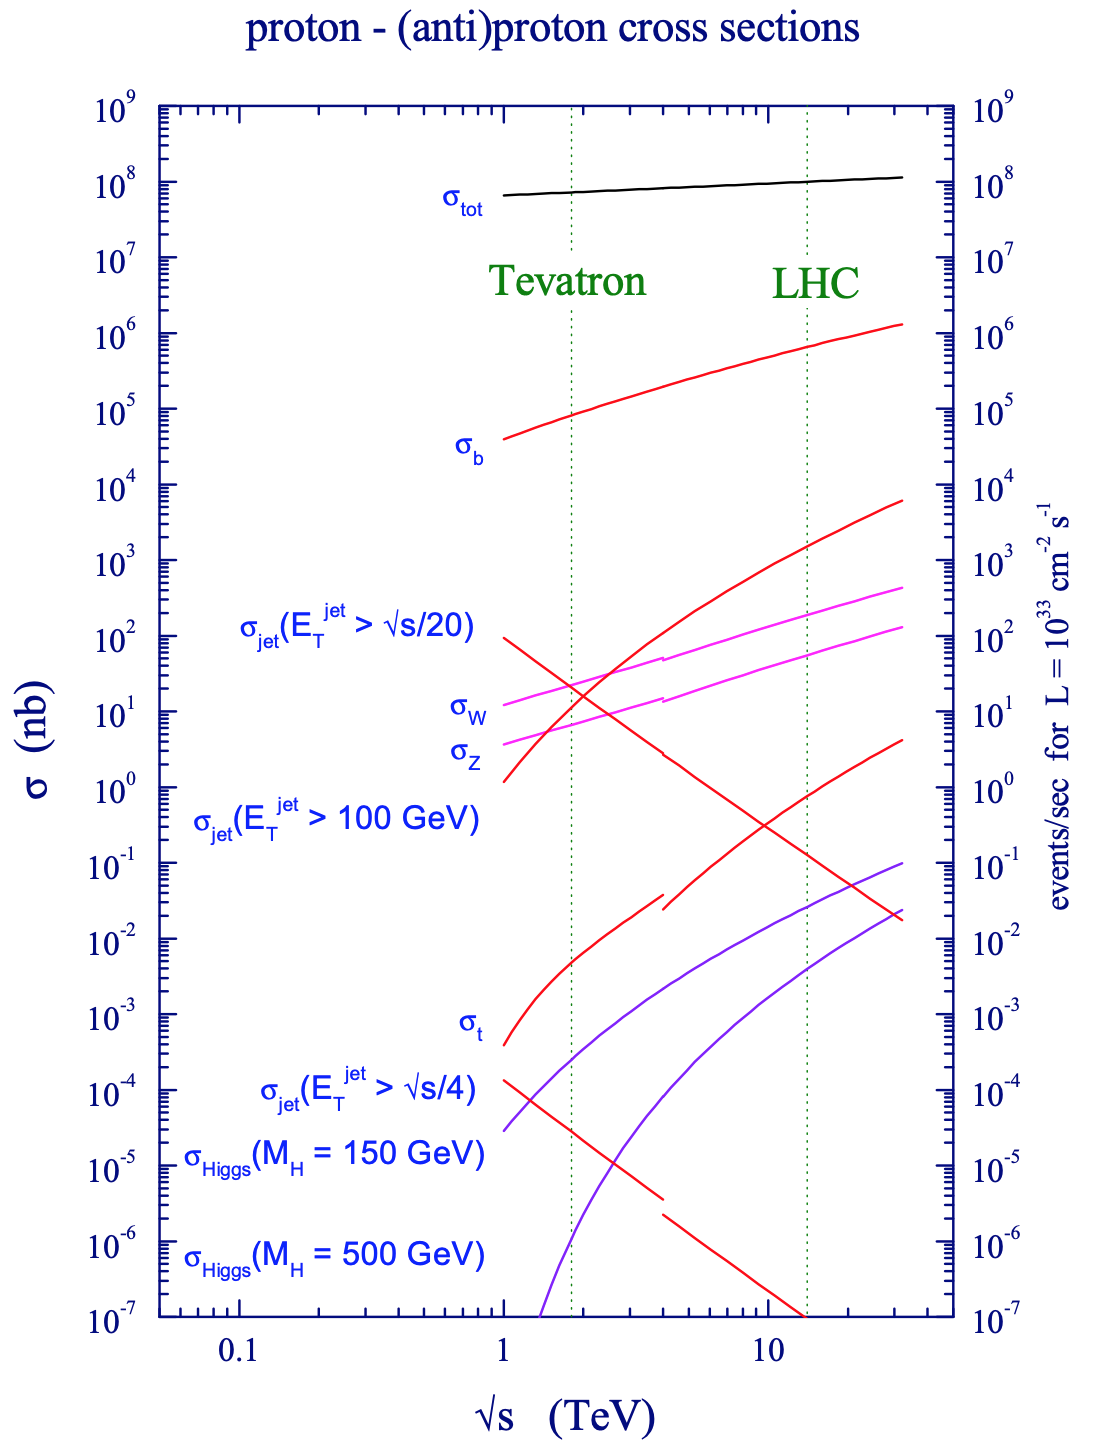
\includegraphics[width=0.6\linewidth]{figures/physics_of_pp/pp_cross_sections.png}
    \caption{Cross sections for typical processes of interest in pp collision experiments, shown as a function of the center-of-mass energy, $\sqrt{s}$. Taken from~\cite{Campbell:2006wx}.}
    \label{fig:pp_xs}
\end{figure}

\subsection{Parton Showers, Hadronization, and Jets} \label{sec:pp_physics_jets}
High energy processes involving the strong interaction are very well-described by perturbative QCD calculations.
However, at lower energies (less than or equal to about 1 GeV), the perturbative appraoch fails to provide an accurate description of the SM phenomena: the strong coupling $\alpha_s$ of QCD becomes close to unity, as shown in Fig.~\ref{fig:pp_qcd_coupling}.
\begin{figure} [htbp!]
    \centering
    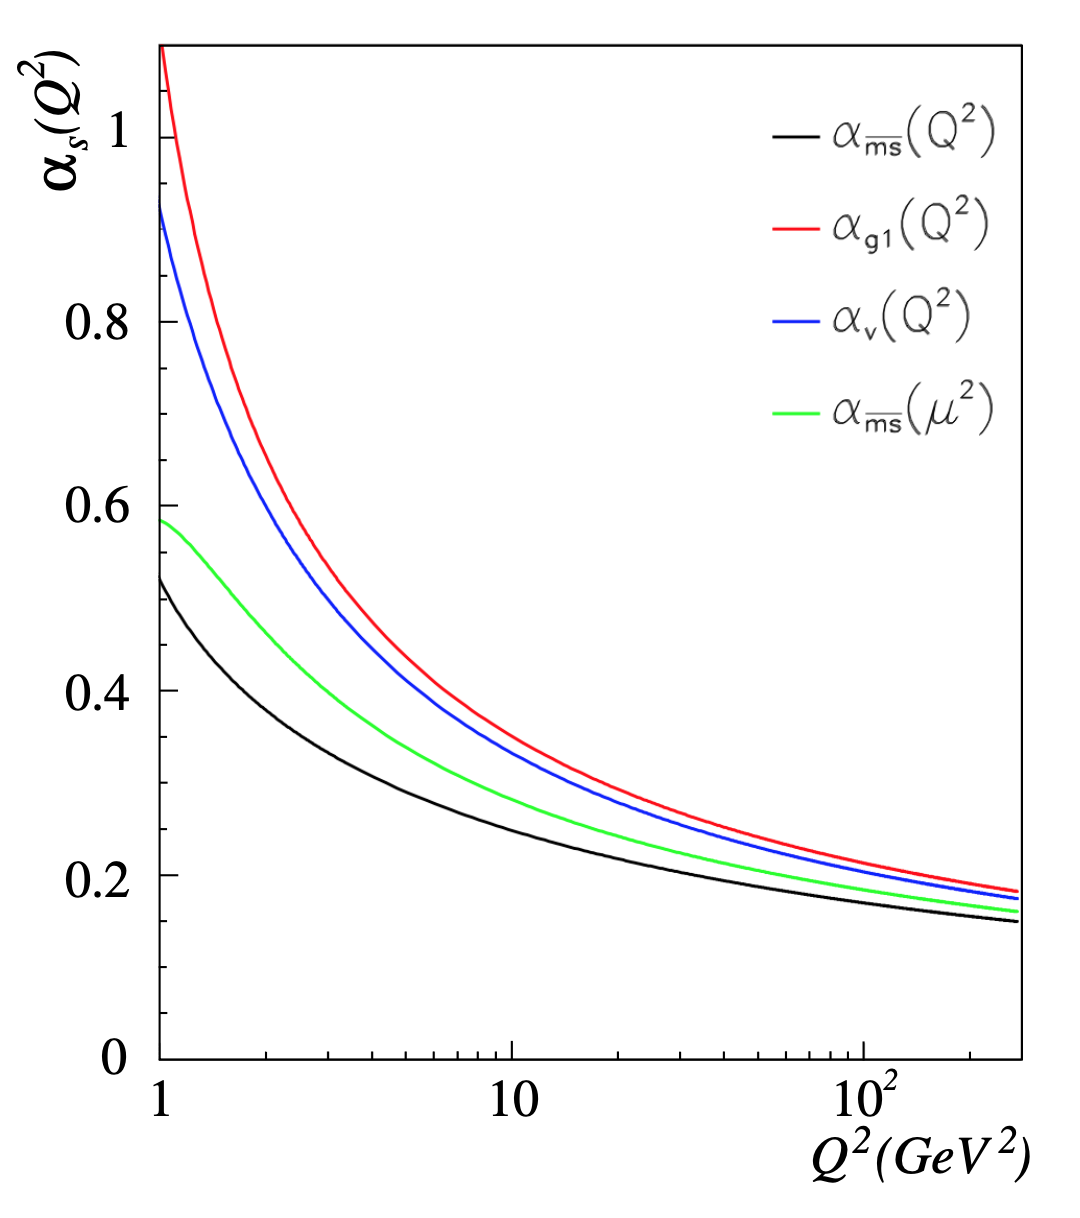
\includegraphics[width=0.6\linewidth]{figures/physics_of_pp/pp_qcd_coupling.png}
    \caption{The strong coupling constant $\alpha_s$ of QCD as a function of $Q^2$. Different colored lines correspond to various renormalization schemes. Taken from~\cite{Deur:2016tte}.}
    \label{fig:pp_qcd_coupling}
\end{figure}
When the coupling $\alpha_s$ nears unity, the perturbative approach fails for the following reason: perturbative expansions are made in powers of the coupling, so the coupling must be significantly less than one in order for a finite expansion to provide a good approximation.
In describing phenomena like parton showers and hadronization, energy scales of $\mathcal O(1)$ GeV are relevant, and a strictly perturbative calculation will not provide a satisfactory description.

A \emph{parton shower} refers to the process by which a high energy parton stemming from the hard interaction produce showers of ``soft'' particles at lower energies.
Typically, this is either gluon splitting, in which a gluon converts into a quark-antiquark pair, or gluon radiation, in which a quark radiates a gluon.
In practice, parton showers are modeled with Monte Carlo generators which utilize Sudakov form factors~\cite{Sudakov:1954sw} and splitting functions to simplify calculations~\cite{Hoche:2014rg}.

As discussed in Sec.~\ref{sec:theory_qcd}, quarks and gluons are confined to bound states which must be colorless.
Moreover, the potential energy of a hadron increases as a function of the distance between the partons.
At a large enough distance, it becomes energetically favorable to break the original bound state in which they existed and instead form new hadrons.
This process is called \emph{hadronization}.
In high energy collisions, quarks and gluons are often ejected from the hard interaction with high enough momentum for hadronization to occur. 
Frequently, the newly formed hadron will initiate a cascade of decays and gluon radiation, forming a cone of hadronic activity.
This cone of particles stemming from the hadronization of a quark or gluon is called a \emph{hadronic jet}.
Hadronization cannot be adequately described through perturbative calculations alone, and instead phenomenological models like the Lund-String Model~\cite{Andersson:1983ia} are employed.

\subsection{Underlying Event and Pileup}
